\Author{\daAuthorTwo}

\subsubsection{Dart}
Dart is a programming language initially designed for web development, with the goal of replacing JavaScript, in mind. Today, it is used in a variety of software products, mainly because of the flutter framework. Dart can be compiled for many platforms and architectures, including ARM, x64, RISC-V, JavaScript or WebAssembly and is highly popular for its combination of high-level features, combined with practical language features like garbage collection and optional type annotation. It was developed by Google and is now an open-source project. \autocite{Flutter:FlutterForBeginners}

\begin{figure} [H]
    \center
    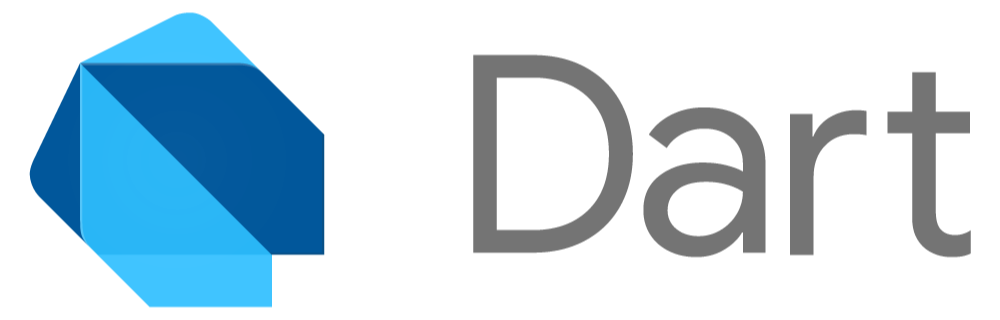
\includegraphics [width=0.6\textwidth] {images/Technologies/dartLogo.png}
    \caption{Dart Logo (Source: \url{https://dart.dev})}
\end{figure}

\subsubsection{Flutter}
Flutter is an open-source software development framework. It allows programmers to compile their applications for different platforms including Web, macOS, iOS as well as Windows and any type of Linux-based systems, all from a single codebase, written in Dart. This allows for more efficient and faster cross-platform development. Another benefit of Google's toolkit is the highly customizable, predefined UI components. Developers can mix and match these components as needed which makes them an applicable choice. \autocite{Flutter:ReadMe}\autocite{Flutter:dagne2019}

We chose flutter mainly for these reasons, but also because of our previous experience with Java to which Dart is quite similar. Through it, we were able to get started quickly, learn what we need along the way. Having a design through the components was also very helpful and saved us some time. 

\begin{figure} [H]
    \center
    
\includegraphics [width=0.4\textwidth] {images/Technologies/flutterLogo.png}
    \caption{Flutter Logo (Source: \url{https://flutter.dev/})}
\end{figure}

\newpage